\documentclass[a4j,12pt]{jreport}
%\documentclass{jreport}
\usepackage[dvipdfmx]{graphicx}
\usepackage[dvipdfmx]{graphics}
\usepackage{amsmath,amssymb}
% \usepackage{amsmath}
%\usepackage{pxjahyper}
\usepackage{here}
\usepackage{algorithm}
\usepackage{algpseudocode}
\usepackage{hhline} 
\usepackage[hang,small,bf]{caption}
\usepackage[subrefformat=parens]{subcaption}
\usepackage{url}
\captionsetup{compatibility=false}
\usepackage{bm}
\def\syaji{ \chapter*{謝辞} \addcontentsline{toc}{chapter}{謝辞}}
\renewcommand{\bibname}{参考文献}
\setlength{\textheight}{\paperheight}
\setlength{\topmargin}{4.6mm}
\addtolength{\topmargin}{-\headheight}
\addtolength{\topmargin}{-\headsep}
\addtolength{\topmargin}{-\headheight}
\addtolength{\textheight}{-60mm}

\setlength{\textwidth}{\paperwidth}
\setlength{\oddsidemargin}{-0.4mm}
\setlength{\evensidemargin}{-0.4mm}
\addtolength{\textwidth}{-50mm}

\begin{document}

%%%%%%%%%%%%%%%%%%%%%
% 表紙
%%%%%%%%%%%%%%%%%%%%%
\thispagestyle{empty}
\begin{center}
\begin{Large}
\vspace*{0.7cm}
{\large 卒業研究論文}\\
\vspace*{2.5cm}
{\bf 流体シミュレーション}\\
\vspace*{7.5cm}
須之内 俊樹\\
学籍番号\hspace*{1zw}19D8102020C\\
\vspace*{2.5cm}
中央大学理工学部情報工学科\hspace*{1zw} 形状情報処理研究室\\
\vspace*{3.0cm}
2023年3月\\
\end{Large}
\end{center}


%%%%%%%%%%%%%%%%%%%%%
% 概要
%%%%%%%%%%%%%%%%%%%%%
\newpage
\renewcommand{\baselinestretch}{1.25} \selectfont
\pagenumbering{roman}


\begin{center} {\large \bf{概 要}} \end{center}

要約には論文の内容を1ページ以内で総括的に述べる.要約の直後に,論文の内容を表す5語程度以内のキーワードを記す.


\vspace{1zw} \noindent
{\bf キーワード: }流体シミュレーション,CG,PIC/FLIP,

%%%%%%%%%%%%%%%%%%%%%
% 目次
%%%%%%%%%%%%%%%%%%%%%
\tableofcontents


\newpage
\pagenumbering{arabic}

%%%%%%%%%%%%%%%%%%%%%
% 1章
%%%%%%%%%%%%%%%%%%%%%
\chapter{概要} \label{chapter:1}

卒業論文は,A4版の用紙に上下左右とも2[cm]の余白を設け,横書きに1段組で作成する.
本文より前に,要約とキーワード,目次を置く.これらが複数ページにわたる場合,ローマ数字のページ番号i, ii, …を付ける.
要約には論文の内容を1ページ以内で総括的に述べる.要約の直後に,論文の内容を表す5語程度以内のキーワードを記す.
本文が開始するページを1ページとし,ページ番号1, 2, …を付ける.
卒業論文のファイル名は“学籍番号.pdf”とする.

本文は,序論,本論,結論に分割する.
序論は本論への導入部分であり,研究の対象,背景,目的,意義等を述べる.
本論は,論旨が明確になるよういくつかの章に分割し,各章に内容が一目でわかるような題名を付ける.
各章は,必要ならば,さらに節に分ける.


結論には,研究の成果や意義その他を総括的に過去形で述べる.
また,研究の成果にかかわる将来の展望や,後継者に委ねたい今後の課題についても述べる.
本文の内容を理解するために不可欠ではあるが,本文に含めると議論の展開がわかりにくくなる内容,たとえば長大な数式の誘導や命題の証明等は,付録に述べる.


卒業論文の書き方は概要のテンプレートに記載されているので,参考にすること.



%%%%%%%%%%%%%%%%%%%%%
% 2章
%%%%%%%%%%%%%%%%%%%%%
\chapter{序論} \label{chapter:2}

流体力学は,計算機が登場する以前は理論の確認をするためには,実際の流体を用いて実験を繰り返さなければならなかったが,計算機が登場してからは,シミュレーションをすることが出来るようになった.計算機を使った流体力学を特別に,数値流体力学(CFD: Computational Fluid Dynamics)と呼び分けることも多い.CFDは実験で得ることが困難な,流れ場全体の詳細な情報を得ることができる.CFDは流体に触れる製品の設計・開発に非常に大きな貢献をした.ここでいう流体とは,空気,ガスなどの気体や,水,土砂の混ざった水,蜂蜜のような粘性がある液体,砂粒などの固体の粒など多岐にわたる.

また,コンピューターグラフィックスにおいても,流体のアニメーションを計算することができるCFDが貢献していて,映像作品やゲームなどで利用されている.コンピューターグラフィックスにおいては,それらしい流体の運動がリアルタイムでシミュレーションできることが重要視される.精度良く計算できることはそこまで重要視されておらず,場合によってはそれらしさのために,現実より大袈裟なシミュレーションをすることもある.
\chapter{非圧縮性流体のシミュレーション} \label{chapter:3}
\section{基礎概念}
\subsection{ナビエ・ストークス方程式} \label{subsec:nabie}
式(\ref{eq:Navie})で表される式を,ナビエ・ストークス方程式とよび,これは流体力学の支配方程式である.非線形二階微分方程式となっており,代数的に一般解を求める事ができない.式(\ref{eq:compressed})は流体の圧縮性条件である.水や砂粒のように圧縮されない流体を扱うときは,流体の密度が常に一定,つまり密度の時間微分が0になり,それに伴い式(\ref{eq:compressed}の左辺の第二項も0になるという,式(\ref{eq:uncompressed1})と,式(\ref{eq:uncompressed})を得る.式(\ref{eq:Navie})と式(\ref{eq:uncompressed})または式(\ref{eq:uncompressed1})を連立することで非圧縮性流体の速度を求めることができる.ナビエ・ストークス方程式を扱う際は,コンピューターで近似解を解析的に求める手法が用いられる.
\begin{equation}\label{eq:Navie}
\frac{\partial}{\partial t}\bm{u}(\bm{x},t) = -(\bm{u}(\bm{x},t) \boldsymbol{\cdot}\nabla)\bm{u}(\bm{x},t)  - \frac{1}{\rho}\nabla p(\bm{x},t) + \nu\nabla^2\bm{u}(\bm{x},t) + \bm{f}
\end{equation}
\begin{equation}\label{eq:compressed}
\frac{D}{Dt}\rho + \nabla\boldsymbol{\cdot}\bm{u}(\bm{x},t) = 0
\end{equation}
\begin{equation}\label{eq:uncompressed1}
\frac{D}{Dt}\rho  = 0
\end{equation}
\begin{equation}\label{eq:uncompressed}
\nabla\boldsymbol{\cdot}\bm{u}(\bm{x},t) = 0
\end{equation}

ここで,$\bm{u}(\bm{x},t)$は,位置$\bm{x}$,時刻$t$での流体の速度ベクトル,$p(\bm{x},t)$は,位置$\bm{x}$,時刻$t$での流体の圧力値,$\rho$は密度,$\nu$は粘性, $\bm{f}$は外力である.式(\ref{eq:Navie})の右辺の第一項を移流項,第二項を圧力項,第三項を粘性項,第四項を外力項とよぶ.移流項は非線形項であり,その他は線形項である.これらを仮の速度$\bm{u}^*$を用いて,線形項を式(\ref{eq:linear}),非線形項を式(\ref{eq:nonlinear})のように分解し,段階的に計算して,各時刻での流速や圧力を計算する方法が用いられている.
\begin{equation}\label{eq:linear}
\bm{u}(\bm{x},t+1) =  \bm{u}^* - \Delta t(\frac{1}{\rho}\nabla p(\bm{x},t) + \nu\nabla^2\bm{u}(\bm{x},t) + \bm{f})
\end{equation} 

\begin{equation}\label{eq:nonlinear}
\bm{u}^* = \bm{u}(\bm{x},t) - \Delta t(\bm{u}(\bm{x},t) \boldsymbol{\cdot}\nabla)\bm{u}(\bm{x},t) 
\end{equation}

解法として,大きく分けて格子法と粒子法がある.

\subsection{格子法} \label{subsec:grid}
格子法とは,流体を扱う空間を正方形の格子に区切り,格子の中心や辺,頂点などに物理量をサンプリングして計算する方法である.区切る格子の数が多いほど精度が良くなり,計算負荷は増加する.格子法の利点として,規則正しく並んだ格子で空間を離散化することで,微分演算を差分法などの単純な方法で近似することができる.欠点として,移流項を近似計算する際に数値拡散が生じてしまうため,移流項の精度があまりよくない.粘性項は以下の移流項の計算によって,移流項の数値拡散として考えることができるので,省かれて計算されることが多い.

\subsubsection{格子法における移流項の計算} \label{subsec:gridadvect}
$$\frac{\partial}{\partial t}\bm{u}(\bm{x},t) = -\bm{u}(\bm{x},t)\frac{\partial}{\partial \bm{x}}\bm{u}(\bm{x},t)$$
偏微分演算子を風上差分$\frac{\partial}{\partial \bm{x}}\bm{u}(\bm{x},t) = \frac{\bm{u}(\bm{x}+\Delta \bm{x},t) - \bm{u}(\bm{x},t)}{\Delta \bm{x}}$を用いて離散化すると,
$$\frac{\partial}{\partial t}\bm{u}(\bm{x},t) =  -\bm{u}(\bm{x},t)\frac{\bm{u}(\bm{x}+\Delta \bm{x},t) - \bm{u}(\bm{x},t)}{\Delta \bm{x}}$$
二変数のテーラー展開$f(a+h,b+k) \fallingdotseq \sum\limits_{t=0}^n \frac{1}{t!}(h\frac{\partial}{\partial \bm{x}} + k\frac{\partial}{\partial y})^t f(a,b)$を二次まで行うと,
$$\frac{\partial}{\partial t}\bm{u}(\bm{x},t) = -\frac{1}{2!\Delta \bm{x}}\bm{u}(\bm{x},t)\left( (\bm{u}(\bm{x},t)+\Delta t\frac{\partial}{\partial \bm{x}}\bm{u}(\bm{x},t) + (\Delta \bm{x})^2\frac{\partial^2}{\partial \bm{x}^2}\bm{u}(\bm{x},t) \right)$$
            
$$\frac{\partial}{\partial t}\bm{u}(\bm{x},t) =  -\bm{u}(\bm{x},t)\left(\frac{\partial}{\partial \bm{x}}\bm{u}(\bm{x},t) + \Delta \bm{x}\frac{\partial^2}{\partial \bm{x}^2}\bm{u}(\bm{x},t) \right)$$

$$ \frac{\partial}{\partial t}\bm{u}(\bm{x},t) =  -\bm{u}(\bm{x},t)\frac{\partial}{\partial \bm{x}}\bm{u}(\bm{x},t) -\bm{u}(\bm{x},t)\Delta \bm{x}\frac{\partial^2}{\partial \bm{x}^2}\bm{u}(\bm{x},t)$$

ここで,$ -\bm{u}(\bm{x},t)\Delta \bm{x} = \mu$とし,$\frac{\partial^2}{\partial \bm{x}^2}\bm{u}(\bm{x},t) = \nabla^2\bm{u}(\bm{x},t)$とすれば,

$$ \frac{\partial}{\partial t}\bm{u}(\bm{x},t) =  -\bm{u}(\bm{x},t)\frac{\partial}{\partial \bm{x}}\bm{u}(\bm{x},t) +\mu\nabla^2\bm{u}(\bm{x},t))$$
となり,右辺の二項目が数値拡散となるが、粘性項の形と同じであることがわかる。
\subsubsection{格子法における非線形項の計算} \label{subsec:gridpressure}
式(\ref{eq:linear})の粘性項は先述の通り省略し,外力項は事前に流速に与えておく.残った圧力項の計算について考える.ただし,移流項を先に計算し,$\bm{u}^*$は既知のものとする.
\begin{equation}\label{eq:uncalculated_pressure}
\bm{u}(\bm{x},t+1) =  \bm{u}^* - \frac{\Delta t}{\rho}\nabla p(\bm{x},t)
\end{equation} 
両辺の発散をとると,
$$\nabla\boldsymbol{\cdot}\bm{u}(\bm{x},t+1) =  \nabla\boldsymbol{\cdot}\bm{u}^* - \frac{\Delta t}{\rho}\nabla^2 p(\bm{x},t)$$
流体の非圧縮性条件,$\nabla\boldsymbol{\cdot}\bm{u}(\bm{x},t) = 0$により,左辺は0になるため,
\begin{equation}\label{eq:calculated_pressure}
\nabla\boldsymbol{\cdot}\bm{u}^* = \frac{\Delta t}{\rho}\nabla^2 p(\bm{x},t)
\end{equation} 
この式を満たすような圧力を求め,式(\ref{eq:uncalculated_pressure})に代入することによって,次の時刻の流速$\bm{u}(\bm{x},t+1)$が計算できる.式(\ref{eq:calculated_pressure})のような微分方程式はポアソン方程式と呼ばれ,境界条件が分かれば解が存在することが知られている.ここでいう境界条件とは,扱う領域の境界での$p(\bm{x},t)$の値がわかっていることとなる.
\subsubsection{格子法の物理量のサンプリング方法} \label{subsec:grid_sampling}
\begin{figure}[htbp]
\begin{center}
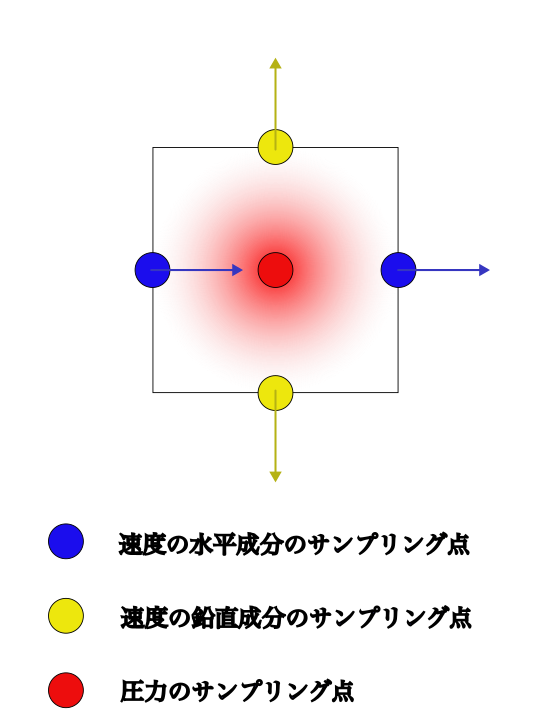
\includegraphics[width=60mm]{staggerd.png}
\caption{スタッガード格子}
\end{center}
\end{figure}

CGの流体シミュレーションにおいて,Fedkiewらの,Marker-And-Cell(MAC)法で格子を離散化する方法がよく用いられている.この手法では,扱う領域を正方形の格子に区切り,圧力を格子の中心に配置する.流速は格子面の中心に,その格子面と垂直な流速の成分を配置する.例えばx-y平面に並行な格子面には,その地点での流速のz成分を配置する.これはスタッガード格子と呼ばれている.この手法は格子点に全ての物理量を配置するコロケート格子と比べ,境界付近の流速が表現しやすく,それらしいシミュレーションができるだけでなく,ポアソン方程式の境界条件の設定も容易である.具体的には,格子が壁に隣接している場合,その面からの流体の流入出はゼロであるため,壁面方向の圧力差と,壁面と隣接している面の中心に配置されている流速成分は共にゼロにする.

スタッガード格子を用いた,格子法の線形項の計算の離散化方法について考える.
$$\nabla\boldsymbol{\cdot}\bm{u}^* = \frac{\Delta t}{\rho}\nabla^2 p(\bm{x},t)$$
スタッガード格子では圧力と流速が配置してある位置がずれているため,両辺に同じ差分を適用できない.離散化する方法として,両辺をセルの領域で積分して考える.
$$\int_V\nabla\boldsymbol{\cdot}\bm{u}^* = \int_V\frac{\Delta t}{\rho}\nabla^2 p(\bm{x},t)$$
両辺にガウスの発散定理を適用すると,周回積分の形で表せる.
$$\oint_V\bm{u}^*\boldsymbol{\cdot}\bm{n} = \oint_V\frac{\Delta t}{\rho}\nabla p(\bm{x},t)\boldsymbol{\cdot}\bm{n}$$
この式はスタッガード格子格子において,周回積分は格子の各面で境界条件を考えて,全ての面の物理量を足すことで表すことができる.
ここで,整数$n=0..5$までを,それぞれ格子の各面の方向に割り振ると,

$$ \sum_{n}\bm{u_n}^*D_nF_n\Delta x = \sum_{n}\frac{\Delta t}{\rho}\nabla p_n(\bm{x},t)F_n\Delta x $$

それぞれの係数は次のようになっている.
\begin{quote}
	\begin{itemize}
		\item $F_n$ 格子の面の各方向に隣接しているものが流体なら1,壁面なら0を取るブーリアン値
		\item $D_n$ 格子の面の各方向に垂直で,格子の外側を向く単位ベクトルを表す係数.向いている方向が軸の正の向きなら+1,					負の向きなら-1を取る整数値.
		\item $p_n$ 割り振られた方向に隣り合っている格子の圧力値.
		\item $u_n$ 割り振られた方向の格子面に配置されている流速値.
	\end{itemize}
\end{quote}

圧力を計算する格子の添字を$(i,j,k)$とし,圧力の微分に前方差分$\nabla \bm{p_n}(\bm{x},t) = \frac{\bm{p_n}(\bm{x},t) - \bm{p_{i,j,k}}(\bm{x},t)}{\Delta \bm{x}}$を適用すると,

$$ \sum_{n}\bm{u_n}^*D_nF_n\Delta x = \sum_{n}\frac{\Delta t}{\rho}\frac{\bm{p_n}(\bm{x},t) - \bm{p_{i,j,k}}(\bm{x},t)}{\Delta \bm{x}}F_n\Delta x $$
式を整理すると,
\begin{equation}\label{eq:discretized_pressure}
\sum_{n}\bm{u_n}^*D_nF_n= \sum_{n}\frac{\Delta t}{\rho}\frac{\bm{p_n}(\bm{x},t) - \bm{p_{i,j,k}}(\bm{x},t)}{\Delta \bm{x}}F_n
\end{equation} 

この式を満たす圧力を求めれば良い.式(\ref{eq:discretized_pressure})は未知数$p$の連立一次方程式となっている.直接法ではなく反復法を用いて,必要な精度で計算を打ち切って計算し,解法としては前処理付き共役勾配法がよく用いられている.

\subsubsection{ディリクレ境界条件} \label{subsec:Dirichlet}
圧力計算の境界条件は,シミュレーションによって追加することもある.ディリクレ境界条件は流体と気体の領域を両方考える際に用いる境界条件で,流体が存在しない格子の圧力値を0とする.
\subsection{粒子法} \label{subsec:particle}
粒子法とは,流体をいくつかの小さな粒子の集まりとして考え,各粒子に物理量を与えて計算をする方法である.本来は流体は,アボガドロ数($N_A = 6.02*10^{23}$)単位の分子が動いているが,これら全てを計算機で扱うのは不可能であるため,いくつかの分子の動きを一つの粒子にまとめて扱う.粒子の数が多いほど実際の現象に近づき,精度が良くなるが,計算負荷は増加する.利点として,以下の計算によって,移流項の計算に数値拡散が発生しないことが確認できるため,移流項が精度良く計算できる.欠点として,その他の微分演算を単純な方法で近似することができないため,その他の項は計算の精度が悪い.
\subsubsection{粒子法における移流項の計算} \label{subsec:particleadvect}
簡単のため,ナビエストークス方程式から粘性項と外力項を取り除いた,オイラー方程式と呼ばれるものについて考える.
$$\frac{\partial}{\partial t}\bm{u}(\bm{x},t) = -(\bm{u}(\bm{x},t)\boldsymbol{\cdot}\nabla)\bm{u}(\bm{x},t) - \frac{1}{\rho}\nabla \bm{p}$$
粒子法はラグランジュ微分を用いることで、移流項の計算が単純になる。
時刻$t_0$に位置$\bm{x_0}$にある流体の速度を$\bm{u}(\bm{x_0},t_0)$とする.$\Delta t$秒後の位置は$\bm{x_0}+v(\bm{x_0},t_0)\Delta t$になっているので,時刻$t_0+\Delta t$の流体の速度は、$\bm{u}(\bm{x_0}+\bm{u}(\bm{x_0},t_0)\Delta t,t_0+\Delta t)$となる。この間の速度変化$\Delta \bm{u}$をテイラー展開を用いて表すと,

$$ \Delta \bm{u} = \bm{u}(\bm{x_0}+v\Delta t,t_0+\Delta t) - \bm{u}(\bm{x_0},t_0) = \frac{\partial \bm{u}(\bm{x_0},t_0)}{\partial \bm{x}}\bm{u}(\bm{x_0},t_0)\Delta t + \frac{\partial \bm{u}(\bm{x_0},t_0)}{\partial t}\Delta t$$

両辺を$\Delta t$で割ると,
$$ \frac{\Delta \bm{u}}{\Delta t} = \frac{\partial \bm{u}(\bm{x_0},t_0)}{\partial \bm{x}}\bm{u}(\bm{x_0},t_0) + \frac{\partial \bm{u}(\bm{x_0},t_0)}{\partial t}$$
$$ \frac{\Delta \bm{u}}{\Delta t} = (\bm{u}\boldsymbol{\cdot}\nabla)\bm{u} + \frac{\partial \bm{u}(\bm{x_0},t_0)}{\partial t}$$

$\frac{\Delta \bm{u}}{\Delta t}$を$\frac{\rm{D}\bm{u}}{\rm{D}t}$と表記し,ラグランジュ微分,または物質微分と呼ぶ.
ラグランジュ微分,つまり,粒子を流れに沿って動かしたときの変化量が,オイラー方程式の移流項になっている.粒子法では,物理量をもった粒子自体を動かすだけで,移流項の計算をすることができる.

\subsubsection{粒子の位置の補正} \label{subsec:fixparticlepos}
粒子を流速に沿って移動させた際,境界をすり抜けてしまうことがある.この対策として,各時刻で,飛び出してしまった粒子を境界内に戻す手法がある.戻す方向や距離は,陰関数を用いたレベルセットサーフェスを考えることで,比較的簡単に実装できる.

粒子法で流体の非圧縮性条件を満たすようなシミュレーションをするには,大きく分けて二つの方法がある.1つはポアソン方程式を解く方法である.MPS法などの粒子法は,格子法でも登場したポアソン方程式を解く方法を取っているが,離散化が格子法のように簡単には行えず,精度や計算時間に問題がある.2つ目は,粒子の密度を計算し,密度が一定になるように粒子を移動させたり,粒子を増減させる方法である.SPH法などはこのような方法をとっている.この方法はナビエストークス方程式の計算過程とは関係ないため,粒子の分布の変化に伴って粒子の物理量も補正する必要がある.一つ目の方法は流体の非圧縮性条件として,式(\ref{eq:uncompressed})を用いているのに対し,二つ目の方法は,式(\ref{eq:uncompressed1})を使っていると考えることもできる.式(\ref{eq:uncompressed1})を利用する手法は確実に密度が保存されるため,密度に関しては頑健であるのに対し,圧力が振動してしまう.それに対し式(\ref{eq:uncompressed})を用いる方法は密度の計算誤差が蓄積していってしまうのに対し,圧力の振動を防ぐことができる.

\section{関連研究} \label{sec:reratedworks}
\subsection{PIC(Particle In Cell)} \label{subsec:PIC}
粒子法は移流項の計算の精度がよく,他の線形項の精度が悪い.格子法は移流項の精度が悪く,他の線形項の精度が良い.OOらの手法は,粒子法と格子法の利点を組み合わせた手法である.粒子と格子の間で物理量を受け渡し,移流項の計算を粒子で行い,その他の計算を格子で行う.
\subsubsection{粒子と格子での物理量の受け渡し} \label{subsec:P2GG2P}
時刻$t$において,格子の周辺にある粒子について,格子の物理量が格納されている位置を$\bm{x}^t_i = (x^t_i,y^t_i)$,粒子の位置を$\bm{x}^t_p$,格子の流速を$\bm{v}^t_i$,粒子の流速を$\bm{v}^t_p$,格子の質量を$m^t_i$,粒子の質量を$m^t_p$とする.ただし,基本的には粒子の質量は時刻によらず一定である.また,格子の一辺の長さを$h$とする.まず,格子と粒子の位置による重みを以下のように定義する.
\begin{equation}\label{eq:weight}
w^t_{ip} = N^t_i(\bm{x}^t_p) = N(\frac{1}{h}(x^t_p - x^t_i))\boldsymbol{\cdot}N(\frac{1}{h}(x^t_p - x^t_i))
\end{equation} 

$N(x)$はカーネル関数であり,以下のように定義する.
\begin{equation}\label{eq:kernel}
N(x) = 
\begin{cases}
\frac{1}{2}|x|^3 - |x|^2 + \frac{2}{3} & (0\leqq|x|<1) \\
\frac{1}{6}(2-|x|)^3 & (1\leqq|x|\leqq2) \\
0 & else.
\end{cases}
\end{equation} 
カーネル関数は,引数の絶対値が0に近いほど大きく,離れるに従って小さくなっていく,微分可能な関数である.粒子と格子の距離が格子の幅の二倍以上離れていると重みは0になるため,その範囲内の粒子についてのみ考えればよい.

次に格子の質量について,以下のように定義する.
\begin{equation}\label{eq:grid_m}
m^t_i = \sum\limits_p m^t_pw^t_{ip}
\end{equation} 

式(\ref{eq:grid_m})を使って,粒子の速度を格子の速度に以下のように受け渡す.

\begin{equation}\label{eq:P2G}
\bm{v}^t_i = \sum\limits_p w^t_{ip}\bm{v}^t_p / m^t_i
\end{equation} 

式(\ref{eq:P2G})は,両辺に$m^t_i$をかけることで運動量についての式になり,シミュレーション全体では運動量が保存しているように振る舞う.

\subsubsection{PICのアルゴリズム} \label{subsec:PIC_algo}
PICの大まかなアルゴリズムは以下のようになる.
\begin{quote}
	\begin{itemize}
		\item 粒子の流速$\bm{v}^{t}_p$を式(\ref{eq:P2G})に従って,格子の流速$\bm{u}(\bm{x},t)$に受け渡す.
		\item 格子の流速に重力等の外力の情報を反映させる.例えば重力は$\bm{u}(\bm{x},t) += \bm{f}\Delta t$のように反映させる.
		\item \ref{subsec:gridpressure}のように,格子法と同じ方法で格子の圧力項を計算する.ここで,格子の次の時刻での流速$\bm{u}_t(\bm{x},t+1)$が求められる.
		\item 格子の次の時刻での流速$\bm{u}(\bm{x},t+1)$を粒子に受け渡し,粒子の次の時刻の流速$p\bm{v}_{t+1}$を求める.この際も式(\ref{eq:P2G})と同様の重みを使用する.
		\item 粒子の位置を$\bm{v}^{t+1}_p$を使って,$\bm{x}^{t+1}_p = \bm{v}^{t+1}_p\Delta t $のように更新する.
	\end{itemize}
\end{quote}

一般的に粒子の数が格子の数よりも多いため,粒子から格子に物理量を受け渡す際に,1つの格子に対して複数の粒子の物理量を集める.この際に,通常の粒子法と比べると粒子の粘性が高くなるような効果がある.これを人工粘性と呼ぶ.格子法とは異なり,移流項を粒子法で計算すると粘性項を別途計算する必要があるが,PICは人工粘性があるため,粘性項は計算しない.しかし,意図しない粘性が含まれてしまうため,粘性の小さな流体のシミュレーションには不向きである.この人工粘性を解決するためのさまざまな手法が提案されている.
\subsection{FLIP(Fluid Implicit Particles)} \label{subsec:FLIP}
PICのアルゴリズムを少し変更し,格子の速度の変化分を粒子に受け渡す.アルゴリズム内では,線形項の計算に入る前に現在の流速を保存しておく.圧力項の計算が終わってから,格子の速度を粒子の速度に受け渡す際に,粒子の速度を直接計算するのでなく,変化分を重みづけして計算し,現在の粒子の速度に加算する.この方法を取ることで,PICのように,格子の影響の範囲内にある粒子の速度が同じような方向に向いてしまうことがなくなる.これにより,PICの人工粘性を解消することができる.問題点として,数値誤差が蓄積し続ける,粒子の勢いがほとんど減衰しないなどがある.実際の流体は粘性が少なからずあるため,粘性を別で考える必要がある.
\subsubsection{PIC/FLIP} \label{subsec:PIC/FLIP}
FLIPの粘性を考える際,PICで計算した速度の影響を少しだけ入れることで,人工粘性を持たせる方法である.PICで計算した速度を$\bm{v}_{\rm{PIC}}$,FLIPで計算した速度を$\bm{v}_{\rm{FLIP}}$とすると,$\bm{v}_{\rm{PIC/FLIP}}$ は以下のように計算する.

\begin{equation}\label{eq:PIC/FLIP}
\bm{v}_{\rm{PIC/FLIP}} =\alpha \bm{v}_{\rm{FLIP}} +(1-\alpha) \bm{v}_{\rm{PIC}}
\end{equation} 

ここで$\alpha$は0から1までの係数で,小さくするほどPICの速度の割合が大きくなり,粘性が大きくなる.
しかし,FLIPの数値誤差が蓄積する問題は解決しておらず,PICの角運動量や運動エネルギーが失われてく問題も残っている.

\subsubsection{PIC/FLIPの粒子位置の修正}\label{subsubsec:fixparticlepos}
\ref{subsec:fixparticlepos}で粒子法における粒子位置の修正法を紹介したが,PIC/FLIPは圧力項を粒子法で計算しないため,ポアソン方程式を解く方法を使用するのは手間である.そのため,式(\ref{eq:uncompressed1})のように,密度が一定になるように直接補正する方法を紹介する.まず,全ての粒子について,粒子の密度分布を修正する方向ベクトル$\Delta p_i$を計算する.
\begin{equation}\label{eq:w_smooth}
W_{smooth}(\bm{r},h) = max(0,1-||r||^2/h^2)
\end{equation} 

\begin{equation}\label{eq:w_sharp}
W_{sharp}(\bm{r},h) = max(0,h^2/||r||^2 - 1)
\end{equation} 

\begin{equation}\label{eq:fixVector}
\Delta p_i = -\gamma \Delta td_i\sum\limits_j \frac{p_j - p_i}{||p_j - p_i||}W_{smooth}(p_j - p_i,d_i)
\end{equation} 

ここで,$W_{smooth}$は平滑化カーネルで,$W_{sharp}$は中心で値が無限大になるようなカーネルである,$\gamma$は修正度合いを表す係数で,$d_i$は粒子半径である.$p_i$,$p_j$は粒子の位置である.このベクトルに従って粒子の位置を$x_p += \Delta p_i$のように修正する.次に,粒子の物理量をそのままに,粒子の位置を修正すると,粒子によって表現されている流体の物理量の分布が歪んでしまうため,粒子の物理量も計算し直す必要がある.粒子$i$の物理量$q(\bm{p_i})$ は以下のように修正する.
\begin{equation}\label{eq:fixVelocity}
q(\bm{p_i}) = \frac{\sum\limits_j m_jq_jW_{sharp}(p^*_j - p_i,d_i)}{\sum\limits_j m_jW_{sharp}(p^*_j - p_i,d_i)}
\end{equation} 

ここで,$q_j,m_j,p^*$はそれぞれ,粒子の物理量,粒子の質量,修正前の粒子の位置である.この手法による粒子位置の修正は,PICのように角運動量や運動エネルギーが失われてく性質があるため,視覚的には人工粘性が大きくなるような効果がある.
\subsection{MPS法における不自然な数値振動の抑制}\label{subsec:japan}
\ref{subsec:fixparticlepos}で述べたように,流体の非圧縮性条件に従った粒子位置の修正方法には種類があり,それぞれ利点と欠点がある.PICが格子法と粒子法を混ぜ合わせて計算しており,PIC/FLIPがPICとFLIPを混ぜ合わせて計算しているように,粒子位置の修正方法を混ぜ合わせた手法となっている.圧力振動がある手法は密度変化をよく防止するため,緩和して用いることができるこの手法によって,既存の他の手法よりも安定した計算と,なめらかな圧力分布を実現している.
\chapter{提案手法} \label{chapter:4}
\section{FLIPの実装} \label{sec:ImpFLIP}
まず,PIC/FLIPの実装方法について考える.本手法では二次元,三次元のデータを扱うため,c++の線形代数ライブラリ,Eigenを用いる.
スタッガード格子の水平方向の数を$Nx$,鉛直方向の数を$Ny$とすると,スタッガード格子は水平方向の速度,鉛直方向の速度,圧力を二次元配列に保存することで実装できる.その際の配列のサイズは以下のようになる.
\begin{quote}
	\begin{itemize}
		\item $水平方向の速度 u[Nx+1][Ny]$ 
		\item $鉛直方向の速度 v[Nx][Ny+1]$ 
		\item $圧力 p[Nx][Ny]$
	\end{itemize}
\end{quote}
粒子から格子に速度を受け渡す際や,外力の影響を考える際に,格子の質量が必要である.この質量は,水平方向と鉛直方向それぞれの速度がサンプリングされている位置と同じ位置に配置する.また,外力は質量と同じ位置での圧力値を二次元配列で与えるが,重力のような保存力を考える場合,格子にかかる力は格子の質量によって異なるため,加速度のみを二次元配列で与え,必要に応じて重力を乗算する.また,後にFLIPで流速の変化量を計算するために,変化前の流速を保存する配列を同時に用意する.
粒子については,1つの粒子を,粒子の位置,速度,PICで計算した速度,FLIPで計算した速度をメンバ変数にもつ構造体で実装し,その構造体の配列で全粒子を管理する.
粒子は,実装するシミュレーションの次元を$d$とすると,1つの格子に$2^d$個配置することが多い.つまり,粒子数は二次元の場合だと4NxNyとなる.ここまでをシミュレーションの前に初期化する.

粒子-格子での物理量の受け渡しの際に,格子のサンプリング点の周辺にある粒子を探索する必要がある.粒子の位置を,格子の数と格子の一辺の長さをかけた数で割ることで,粒子がどの格子の近くにあるか判定することができるが,ナイーヴに格子ごとに近傍の粒子を探索
して実装すると,計算量が大きくなってしまう.この問題は,格子ごとにどの粒子が入っているのかを保存するようなデータ構造を,各タイムステップで更新することで解決できる.各タイムステップの最後で粒子の位置を移動させるため,各タイムステップの最初でこのデータ構造を更新する.本手法では   を使用している.c++ではunorderedmapのキーを格子の位置,値を格子に格納されている粒子にすることで実装できる.

次は粒子の速度を格子にわたす.格子点ごとに,カーネル関数の値が非ゼロになるような範囲内の粒子を探索し,式(\ref{eq:P2G})を用いて格子の速度を計算する.例えばカーネル関数として,式(\ref{eq:kernel})を利用するとすると,計算している格子の,このとき,粒子の速度のうち,速度を保存している配列の,保存している速度成分のみを受け渡す.同時に格子の質量も計算される.FLIPで,後に速度の変化量を計算するため,この段階で計算した速度を保存する.

\section{圧力項の離散化と実装} \label{sec:Imppressure}
\begin{equation}\label{eq:discretized_pressure}
\sum_{n}\bm{u_n}^*D_nF_n= \sum_{n}\frac{\Delta t}{\rho}\frac{\bm{p_n}(\bm{x},t) - \bm{p_{i,j,k}}(\bm{x},t)}{\Delta \bm{x}}F_n
\end{equation}

圧力項は圧力を変数とした,上記の連立方程式を解く.連立方程式を$\bm{Ax=b}$とすると係数行列$\bm{A}$と,係数行列$\bm{b}$は以下のように計算する.また,それぞれのサイズは,格子の総数を$n$とすると,$\bm{A}$は$n \times n$であり,$\bm{b}$は$n$である.
\begin{quote}
	\begin{itemize}
		\item 全粒子について,ディリクレ境界条件を考える.これは先ほどのデータ構造で粒子が格納されていない格子の圧力の係数を0にすることで実装できる.
		\item 格子の流速に重力等の外力の情報を反映させる.例えば重力は$\bm{u}(\bm{x},t) += \bm{f}\Delta t$のように反映させる.
		\item \ref{subsec:gridpressure}のように,格子法と同じ方法で格子の圧力項を計算する.ここで,格子の次の時刻での流速$\bm{u}_t(\bm{x},t+1)$が求められる.
		\item 格子の次の時刻での流速$\bm{u}(\bm{x},t+1)$を粒子に受け渡し,粒子の次の時刻の流速$p\bm{v}_{t+1}$を求める.この際も式(\ref{eq:P2G})と同様の重みを使用する.
		\item 粒子の位置を$\bm{v}^{t+1}_p$を使って,$\bm{x}^{t+1}_p = \bm{v}^{t+1}_p\Delta t $のように更新する.
	\end{itemize}
\end{quote}
\section{シミュレーション領域の定義} \label{sec:levelsetserface}
本手法では,シミュレーションは正方形の内部の領域内で行う.正方形の一辺の長さ$L$は,スタッガード格子の水平方向の数を$N$,スタッガード格子の一辺の長さを$dx$とすると,$L = Ndx$である.
4点$(0,0),(L,0),(0,L),(L,L)$を頂点とするような正方形のレベルセットサーフェス$\varphi(x,y)$を,以下のように定義する.
\begin{equation}\label{eq:levelsetserface}
\varphi(x,y)
\begin{cases}
(x,y) & x \le0 , y \le 0\\
(L - x,y) & L \le x , y \le 0\\
(x,L-y) & x \le0 , L \le y)\\
(L-x,L-y) & L \le x , L \le y)\\
(0,0) & else\\
\end{cases}
\end{equation} 
このようにして定義されるレベルセットサーフェスは,粒子の座標を引数とし,4点$(0,0),(L,0),(0,L),(L,L)$を頂点とするような正方形から外に出ていだ場合は,正方形領域に最短距離で戻すようなベクトルを返り値として返す.粒子に対して移流計算や粒子位置の補正を行うと,シミュレーション領域から粒子が出ていってしまうことがあるため,そのような計算を行った後に全粒子に対して領域内部に戻す処理を行う.

\section{シミュレーションの定数や,カーネル関数の決定} \label{sec:constant}
流体シミュレーションにおけるさまざまな定数や,カーネル関数は,シミュレーションしたい流体や,シミュレーションの手法によってどのような値を用いるのが最適かは異なっている.
\chapter{計算機実験} \label{chapter:5}

一例として,和文の著書\cite{suetake},和文の論文誌\cite{kusano},英文の編書\cite{fuortes},
英文の論文誌\cite{rice},国際会議\cite{guibas},修士論文\cite{chudai},電子雑誌\cite{iwama},Webページ\cite{IPSJ}を,
2ページの参考文献の節に載せる.{\em 参考文献には信頼性が高く,後世に残るものを載せるように注意せよ.}

書くべき情報は以下のとおりである.
\begin{itemize}
\item 和文の著書: 著者,書名,シリーズ名(あれば),発行所,都市,年.
\item 和文の論文誌: 著者,題名,誌名,巻,号,頁,年.
\item 英文の編書: 編者,書名,発行所,都市,年.
\item 英文の論文誌: 著者,題名,誌名,巻,号,頁,年.
\item 国際会議: 著者,題名,予稿集名,都市,コード等,頁,年.
\item 修士論文: 著者,題名,機関名,年.
\item 電子雑誌: 著者,題名,誌名,巻,号,頁(オンライン),DOI,西暦年.
\item Webページ: 著者,Webページの題名,Webサイトの名称(オンライン)(ただし,著者と同じ場合は省略可),入手先〈URL〉(参照日付).
\end{itemize}
英語の文献はすべて半角文字で書く.参考文献には本文で引用した文献のみ載せる.
情報処理学会の論文誌の原稿執筆案内\cite{IPSJ}も参考になる.

通し番号は,引用順または著者名のアルファベット順に付ける.
文献の引用のしかたは分野ごとに異なるので,{\em 自己流では書かず,当該分野の論文誌などを参考にする}こと.



%%%%%%%%%%%%%%%%%%%%%
% 〇章
%%%%%%%%%%%%%%%%%%%%%
\chapter{結論} \label{chapter:6}

結論には,研究の成果や意義その他を総括的に{\em 過去形}で述べる.



%謝辞
\syaji
\par
本研究を進めるにあたり,大変多くのご指導,ご助言を頂いた
中央大学理工学部情報工学科の中央太郎教授に深く感謝いたします.
また,多大なるご助言,ご協力を頂いた〇〇研究室の皆様には大変お世話になりました.
心から感謝いたします.


%参考文献
\begin{thebibliography}{99}
\addcontentsline{toc}{chapter}{参考文献}

\bibitem{suetake}
近藤雅裕,越塚誠一,MPS法における不自然な数値振動の抑制,日本計算工学会論文集,Paper No.20080015,2008. 

\bibitem{fuortes}
Alexey Stomakhin, Craig Schroeder, Lawrence Chai, Joseph Teran, Andrew Selle, \textit{A material point method for snow simulation}, University of California Los Angeles , ACM Transactions on GraphicsVolume 32, Issue 4, July, 2013.

\bibitem{rice}
W. Rice, A. C. Wine, and B. D. Grain, Diffusion of impurities during epitaxy, \textit{Proc. IEEE}, vol.~52, no.~3, pp.~284--290, 1964.

\bibitem{guibas}
L. J. Guibas and R. Sedgewick, A dichromatic framework for balanced trees, 
\textit{Proc. 19th IEEE Sympos. Found. Comput. Sci.}, Ann Arbor, pp.~8--21, 1978.

\bibitem{chudai}
中大次郎,マルチメディアと数理工学,中央大学大学院理工学研究科情報工学専攻修士論文,1998.

\bibitem{iwama}
K. Iwama, A. Kawachi, and S. Yamashita, Quantum biased oracles, \textit{IPSJ Digital Courier}, vol.~1, pp.~461--469 (online), DOI: 10.2197/ipsjdc.1.461, 2005.

\bibitem{IPSJ}
情報処理学会,論文誌ジャーナル(IPSJ Journal)原稿執筆案内,情報処理学会(オンライン),入手先〈\url{https://www.ipsj.or.jp/journal/submit/ronbun_j_prms.html}〉(参照2022-04-25).


\end{thebibliography}

%関連論文, 仕様はthebibliographyと同一. 
%\begin{therelatedreference}{99}
%\end{therelatedreference}
\end{document}